% Provenance (never printed): see sources/outline_sources.md (Year 1: solute and particle
% fluxes; the Hjulstrom diagram; settling velocity; denudation rates). Exercise and problem
% values in the Book 3 scratch calculator calc/ch20.py; figure data from
% figdata/bachelor-1/settling.py and threshold.py. Erosion, transport and deposition are
% Book 1's (g5); the sediment load in three forms, the denudation rate and isostatic rebound
% are Book 2's (g12), re-founded here (load, denudation rate) or recalled (rebound); discharge
% and the drainage basin are Book 2 g10's; Airy isostasy is ch. 11's; viscosity, Stokes' law
% and the Reynolds number are the physics books' (admitted, pointer). Grain-size classes and
% sorting belong to ch. 21.
\chapter{التعرية والنقل}\label{ch:b1:erosion-transport}

بعد عاصفة يصير النهر تحت الجسر بنّيًّا. فالماء الذي كان صافيًا قبل يوم صار كثيفًا بالطين، يدور حول الأعمدة ويحمل الأغصان، وفي القاع، بعيدًا عن الأنظار، تصطدم الحصى ببعضها وهي تتدحرج. وفي كل ثانية يحمل الفيضان أطنانًا من الأرض معه. وفي اتجاه المصبّ، خلف سدّ، يستقرّ الطين نفسه في الماء الساكن للخزّان، الذي يفقد قليلًا من حجمه كل سنة؛ وأبعد من ذلك، عند مصبّ النهر، ينتشر في البحر كعمود بنّي يُرى من الفضاء. يضع هذا الفصل أرقامًا على تلك الرحلة: كم يحمل النهر، وفي أيّ أشكال؛ وكم بسرعة يهبط الحبّة؛ وأيّ تيار يحرّكها أول مرة؛ وكم بسرعة، في النهاية، تُبرى منطقة كاملة.

\begin{recall}
التعرية هي تآكل الأرض ونقل فتاتها بعيدًا؛ والترسيب وضع هذا الفتات حيث يتباطأ الناقل (الكتاب الأول، الصف الخامس). ويحمل النهر حمولته الرسوبية كحمولة قاعية، وحمولة معلّقة، وحمولة مذابة؛
\omterm{def:b1:erosion-transport:denudation}{ومعدّل التعرية} لمنطقة هو سمك الصخر المُزال منها في وحدة الزمن، بالأمتار لكل مليون سنة؛ وحين تزيل التعرية سمكًا قدره $e$ من \omterm{def:b1:layered-earth:layers}{القشرة}، فإن الارتداد الإيزوستاتي لا يجعل السطح يهبط إلا بمقدار $e(1 - \rho_c/\rho_m)$ (الكتاب الثاني، الصف الثاني عشر). وتصريف النهر هو حجم الماء الذي يعبر مقطعًا في وحدة الزمن، وحوضه الصبّي هو المساحة التي تغذّيه (الكتاب الثاني، الصف العاشر).
وفي التوازن الإيزوستاتي لإيري تطفو \omterm{def:b1:layered-earth:layers}{القشرة} على \omterm{def:b1:layered-earth:layers}{الوشاح} بجذر يتناسب مع تضاريسها (\cref{prop:b1:isostasy-gravity:airy}). \omterm{def:b1:weathering-clays:hydrolysis}{والتحلّل المائي} للسيليكات يرسل الأيونات والسيليكا المذابة إلى الأنهار (\cref{def:b1:weathering-clays:hydrolysis}).
اللزوجة الديناميكية $\mu$ لمائع تقيس مقاومته للقصّ، واللزوجة الحركية $\nu = \mu/\rho$؛ وكرة قطرها $d$ تتحرّك ببطء بالسرعة $w$ عبر مائع تشعر بالسحب $3\pi\mu d w$ (قانون ستوكس)؛ وعدد رينولدز $w d/\nu$ يقارن القصور بالقوى اللزجة، وجريان الماء حول الكرة يكون ناعمًا ما دامت صغيرة (كتب الفيزياء).
\end{recall}

\section{تدفّقات المحلول والجسيمات}\label{sec:b1:erosion-transport:fluxes}

يزيل النهر الأرض بطريقتين: كمادة في المحلول، وهي نواتج \omterm{def:b1:weathering-clays:weathering}{التجوية الكيميائية}، وكحبيبات صلبة، وهي نواتج \omterm{def:b1:weathering-clays:weathering}{التجوية الفيزيائية} والبقايا غير القابلة للذوبان من \omterm{def:b1:weathering-clays:weathering}{التجوية الكيميائية}. ويسير الاثنان بطريقتين مختلفتين، والحبيبات نفسها تسير بطريقتين.

\begin{definition}[الحمولة المذابة، والحمولة المعلّقة، والحمولة القاعية]\label{def:b1:erosion-transport:load}
حمولة النهر هي المادة التي يحملها عبر مقطع، في ثلاثة أجزاء تختلف بطريقة سيرها. \emph{الحمولة المذابة}\index{الحمولة المذابة} هي المادة في المحلول، من أيونات وسيليكا مذابة، تتحرّك مع الماء بسرعته. و\emph{الحمولة المعلّقة}\index{الحمولة المعلّقة} تتكوّن من حبيبات يُبقيها الجريان معلّقة بفعل اضطرابه، وأغلبها طين وطمي ورمل ناعم، تتحرّك بسرعة الماء تقريبًا ونادرًا ما تمسّ القاع. و\emph{الحمولة القاعية}\index{الحمولة القاعية} تتكوّن من حبيبات تتدحرج أو تنزلق أو تقفز على القاع، تلامسه كثيرًا، وتتحرّك أبطأ بكثير من الماء.
\end{definition}

\begin{omfigure}
\begin{tikzpicture}[font=\footnotesize, >={Stealth[length=4pt]}]
% schematic: the three loads of a river (side view) and the forces on a bed grain
\fill[omDef!12] (0,0) rectangle (9,3.2);
\draw[omDef!80!black, thick] (0,3.2) -- (9,3.2);
\node[anchor=south west, omDef!80!black] at (0,3.2) {سطح الماء};
% flow profile arrows (velocity grows upward)
\foreach \y/\l in {0.35/0.5, 0.8/0.9, 1.4/1.15, 2.1/1.3, 2.8/1.4} {\draw[->, black!55] (0.25,\y) -- ++(\l,0);}
\draw[black!55] (0.25,0.12) -- (0.25,3.05);
\node[anchor=north west, black!65, align=left] at (0.2,-0.15) {ملف سرعة\\ الجريان};
% bed
\fill[black!12] (0,-0.05) rectangle (9,0.12);
\foreach \x in {0.1,0.45,...,8.9} {\fill[black!45] (\x,0.0) circle[radius=0.09];}
% dissolved load: ions
\foreach \x/\y/\s in {2.3/2.7/+, 3.1/1.9/-, 4.0/2.85/+, 4.7/2.2/-, 5.6/2.75/+, 6.3/1.85/+, 7.2/2.6/-, 8.2/2.2/+, 2.7/1.2/-, 7.8/1.3/-} {\node[circle, draw=omThm, inner sep=0.2pt, minimum size=7pt, font=\tiny, text=omThm] at (\x,\y) {$\s$};}
% suspended load: fine grains, denser near the bed
\foreach \x/\y in {2.1/1.5, 2.6/0.9, 3.0/2.5, 3.4/0.6, 3.7/1.4, 4.2/0.8, 4.4/1.9, 4.9/0.55, 5.2/1.2, 5.5/2.1, 5.9/0.7, 6.1/1.5, 6.6/0.9, 6.9/2.3, 7.4/0.6, 7.6/1.7, 8.0/0.85, 8.5/1.4, 3.9/0.45, 5.0/0.35, 6.4/0.4, 2.4/0.45, 8.6/0.5} {\fill[brown!75!black] (\x,\y) circle[radius=0.05];}
% bed load: rolling and hopping grains
\fill[black!60] (3.2,0.27) circle[radius=0.15];
\draw[->, black!70] (3.0,0.55) arc[start angle=150, end angle=30, radius=0.25];
\fill[black!60] (5.6,0.25) circle[radius=0.12];
\draw[->, black!70, densely dashed] (4.6,0.2) .. controls (4.9,0.9) and (5.3,0.7) .. (5.55,0.4);
\fill[black!60] (4.6,0.22) circle[radius=0.06];
% labels
\node[omThm, anchor=west] at (9.2,2.5) {الحمولة المذابة: أيونات};
\node[brown!75!black, anchor=west] at (9.2,1.5) {الحمولة المعلّقة:};
\node[brown!75!black, anchor=west] at (9.2,1.1) {طين، وطمي، ورمل ناعم};
\node[black!75, anchor=west] at (9.2,0.4) {الحمولة القاعية: تدحرج،};
\node[black!75, anchor=west] at (9.2,0.0) {انزلاق وقفز للحبيبات};
\draw[->, thick, black!70] (6.8,3.55) -- node[above] {الجريان} (8.6,3.55);
% inset: forces on a grain resting on two others; it pivots about its downstream contact
\begin{scope}[xshift=11.8cm, yshift=-2.2cm]
  \fill[black!12] (-1.2,-0.4) rectangle (1.2,0);
  \fill[black!40] (-0.6,-0.15) circle[radius=0.28]; \fill[black!40] (0.6,-0.15) circle[radius=0.28];
  \fill[black!65] (0,0.166) circle[radius=0.4];
  \draw[->, thick, omDef!80!black] (0,0.166) -- (0,1.15) node[above] {الرفع};
  \draw[->, thick, omThm] (0,0.166) -- (1.05,0.166) node[right] {السحب};
  \draw[->, thick, black] (0,0.166) -- (0,-0.8) node[below] {الوزن المغمور};
  \draw[->, thick, black!60] (-1.4,0.85) -- (-0.5,0.85) node[pos=0, left] {الجريان};
  \fill[red!60!black] (0.353,-0.020) circle[radius=0.045];
  \node[font=\scriptsize, anchor=north west, black!70] at (0.5,-0.4) {المحور};
\end{scope}
\end{tikzpicture}

{\small الحمولات الثلاث لنهر، مرئيةً من الجانب (تخطيطية، غير مرسومة بالمقياس). الجريان أسرع قرب السطح ويتباطأ حتى ينعدم عند القاع. والأيونات منتشرة في كامل العمق؛ والحبيبات المعلّقة تحملها الدوّامات، وأكثرها قرب القاع؛ وحبيبات \omterm{def:b1:erosion-transport:load}{الحمولة القاعية} تتدحرج أو تنزلق أو تقفز قفزات قصيرة. وإلى اليمين: القوى على حبيبة من القاع. يميل السحب والرفع للجريان إلى تدحرجها فوق جارتها في اتجاه المصبّ، حول نقطة \omterm{def:b1:geological-maps:geological-map}{التماس}؛ ووزنها في الماء يمسكها.}
\label{fig:b1:erosion-transport:loads}
\end{omfigure}

الحدّ بين الحمولتين الصلبتين لا تحدّده حجم الحبيبة: بل يتوقّف على الجريان. فالفيضان الذي يحمل الرمل معلّقًا يتركه على القاع، كحمولة قاعية، عندما ينحسر؛ أما أدقّ الطين، فيبقى معلّقًا في أيّ تيار تقريبًا، ونادرًا ما يُوجد على قاع نهر جارٍ. وتُقاس كل حمولة كتدفّق، أي كتلة في وحدة الزمن عبر مقطع النهر.

\begin{proposition}[تدفّق حمولة]\label{prop:b1:erosion-transport:flux}
ليكن $c$ تركيز حمولة مذابة أو معلّقة (كتلة في وحدة حجم الماء)، و$u$ سرعة الماء، وكلاهما يتغيّر عبر المقطع الذي مساحته $A$. (1) التدفّق اللحظي للحمولة عبر المقطع هو
\[
  F = \iint_A c\,u\,\mathrm dA = \overline{c}_Q\,Q,
\]
حيث $Q = \iint_A u\,\mathrm dA$ هو التصريف، و$\overline{c}_Q$ التركيز المتوسّط المرجّح بالسرعة. (2) خلال فترة $T$ يتغيّر فيها التصريف $Q(t)$ والتركيز $C(t)$ للنهر، فإن الكتلة المحمولة هي
\[
  M = \int_0^T Q\,C\,\mathrm dt = T\left(\overline{Q}\;\overline{C} +
  \operatorname{cov}(Q, C)\right),
\]
حيث الأشرطة تعني المتوسطات الزمنية، و$\operatorname{cov}(Q, C)$ هو المتوسط ل$(Q - \overline{Q})(C - \overline{C})$. وجداء التصريف المتوسّط والتركيز المتوسّط يعطي الكتلة الصحيحة فقط إذا كان الاثنان غير مترابطين.
\end{proposition}

\begin{proof}
(1) في زمن $\mathrm dt$ يملأ الماء العابر لمساحة صغيرة $\mathrm dA$ من المقطع حجمًا $u\,\mathrm dA\,\mathrm dt$، يحمل الكتلة $c\,u\,\mathrm dA\,\mathrm dt$؛ وجمع ذلك على المقطع يعطي $F$، و$\overline{c}_Q$ معرّف بأنه $F/Q$. (2) نكتب $Q = \overline{Q} + Q'$ و$C =
\overline{C} + C'$، حيث للتقلّبات $Q'$ و$C'$ متوسط صفري خلال الفترة. فيكون $QC = \overline{Q}\,\overline{C} + \overline{Q}\,C' + Q'\,\overline{C}
+ Q'C'$؛ والحدّان الأوسطان يتوسّطان إلى الصفر، ومتوسط $Q'C'$ هو التغاير.
\end{proof}

والتغاير يهمّ للحمولة المعلّقة. فتركيزها يرتفع بحدّة في الفيضانات، حين يغسل المطر التربة إلى المجاري ويرفع الجريان الأسرع الحبيبات من القاع، فيكبر $Q$ و$C$ معًا: فجزء كبير من الرسوب السنوي لنهر يمرّ في أيام قليلة من الفيضان، وحملة أخذ عينات تفوّتها، أو تركيز متوسط مضروب في التصريف المتوسط، تقلّل من الحمولة. أما \omterm{def:b1:erosion-transport:load}{الحمولة المذابة} فتسلك العكس: فالفيضانات تخفّفها، وتركيزها أعلى ما يكون عند الجريان الضعيف، حين يتغذّى النهر من الماء الجوفي الذي طال اتصاله بالصخر.

\begin{method}[الحمولة السنوية لنهر من القياس]\label{met:b1:erosion-transport:gauging}
\begin{enumerate}
  \item سجّل التصريف باستمرار عند محطة قياس.
  \item خذ عينات من الماء عند تصاريف كثيرة، ومنها الفيضانات، وقِس كتلة الرسوب في اللتر (بالترشيح والوزن) وكتلة كل نوع مذاب.
  \item رجّح التركيزات بالتصريف لحظة أخذ العينة للحصول على التركيز المتوسط المرجّح بالتدفّق، أو ركّب التركيز كدالة للتصريف وطبّقها على السجل كله.
  \item اضرب في الحجم الكلّي للماء في السنة، أو اجمع $Q\,C\,\Delta
        t$ على السجل (\cref{prop:b1:erosion-transport:flux}).
  \item أضف \omterm{def:b1:erosion-transport:load}{الحمولة القاعية}، التي لا تلتقطها عيّنات الماء، من قياسات منفصلة أو كنسبة مقدّرة.
  \item بالنسبة للحمولة المذابة، أزل ما لا يأتي من الصخر: الأملاح التي يجلبها المطر، وبالنسبة للبيكربونات، الكربون المأخوذ من الهواء (\cref{ch:b1:weathering-clays}).
\end{enumerate}
\end{method}

\begin{omfigure}
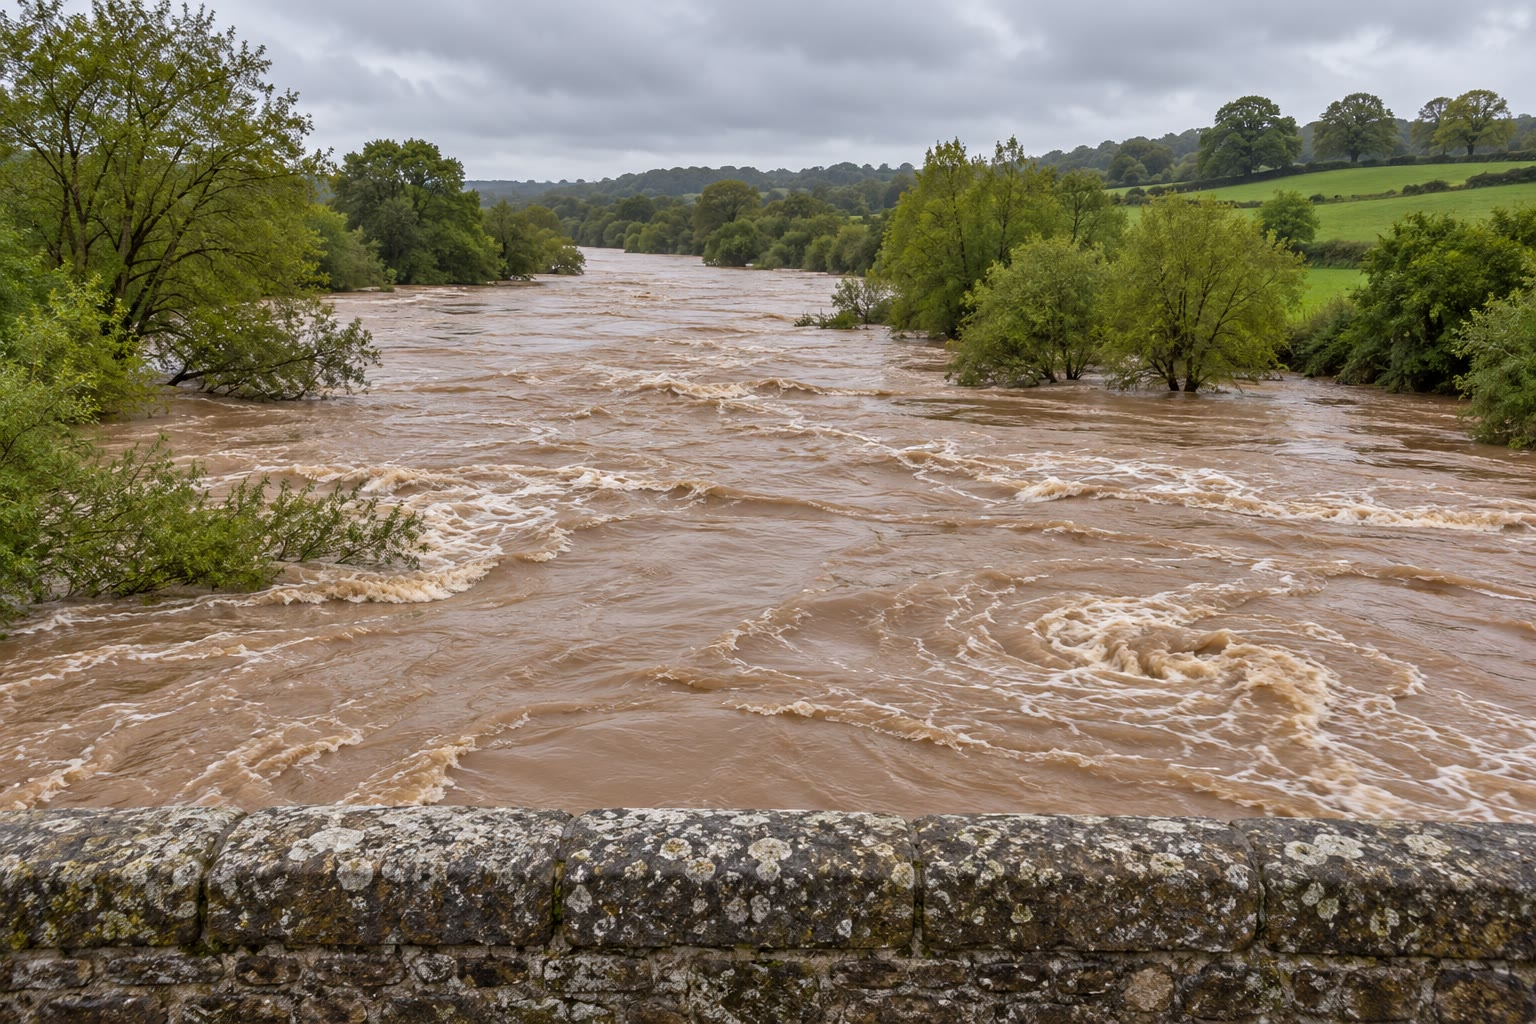
\includegraphics[height=5.1cm]{images/book3/ai/b1-muddy-river.jpg}\hfill
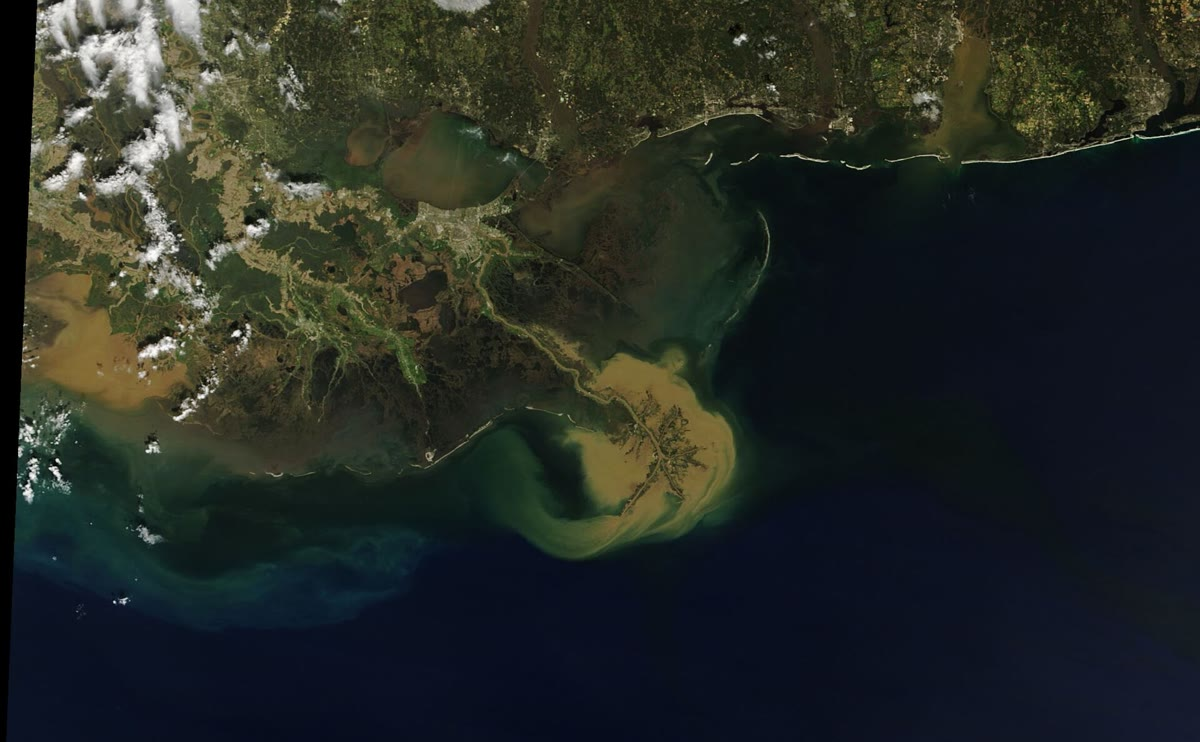
\includegraphics[height=5.1cm]{images/book3/b1-mississippi-plume.jpg}
{\small يسارًا: نهر في فيضان يحمل ماءً بنّيًّا محمّلًا بالرسوب (رسم بالذكاء الاصطناعي). ويمينًا: فيضان نهر المسيسيبي ينسكب في خليج المكسيك حول دلتاه، مرئيًّا بجهاز موديس على القمر الصناعي تيرا في 4 مارس 2018؛ والطين المعلّق يلوّن البحر بنّيًّا وأخضر، والرياح الجنوبية الشرقية تدفع العمود نحو الشمال الغربي. NASA Earth Observatory image by Joshua Stevens, ملك عام، عبر ويكيميديا كومنز.}
\label{fig:b1:erosion-transport:plume}
\end{omfigure}
% ledger: commons:mississippi-plume

\emph{أنهار العالم.} قبل أيّ تأثير بشري، كانت أنهار العالم تحمل نحو \qty{14}{Gt} من الرسوب المعلّق في السنة إلى المحيط الساحلي، و\qty{15.5}{Gt} مع \omterm{def:b1:erosion-transport:load}{الحمولة القاعية}. وغيّر الناس طرفي الرحلة: فالزراعة وإزالة الغابات رفعتا تآكل التربة، فأضافتا نحو \qty{2.3}{Gt} في السنة إلى الأنهار، بينما تحتجز الخزانات الرسوب: فالكبيرة منها تحبس نحو \qty{20}{\percent} من التدفّق، والصغيرة نحو \qty{6}{\percent} أخرى، وأكثر من \qty{100}{Gt} من الرسوب يرقد الآن خلف سدود بُنيت معظمها في الخمسين سنة الماضية. والأثر الصافي نقص: فالتدفّق الحديث نحو \qty{12.6}{Gt} في السنة.
% ledger: syvitski:flux

\begin{dated}{2005}
تأتي أرقام تدفّق الرسوب المعلّق، قبل التأثير البشري وبعده، من نموذج عالمي لرسوب الأنهار نُشر عام 2005. وقد بُنيت سدود منذ ذلك الحين.
\end{dated}
% ledger: syvitski:flux

أما \omterm{def:b1:erosion-transport:load}{الحمولة المذابة} فأصغر. فقد أعطى تجميع كلاسيكي لتحاليل الأنهار، أُنجز عام 1963، أن المادة المذابة التي تسلّمها أنهار العالم إلى البحر تبلغ نحو \qty{3.9}{Gt} في السنة، أي نحو \qty{30}{\percent} من التدفّق المعلّق الحديث، عند تركيز متوسط قدره \qty{120}{mg} في اللتر. والبيكربونات تشكّل نحو نصفها، \qty{58}{mg.L^{-1}}، يليها الكالسيوم والسيليكا والكبريتات والكلوريد والصوديوم. وجزء منها لا يأتي من الصخر: فكثير من البيكربونات يحمل كربونًا مأخوذًا من الهواء أو التربة، وجزء من الكلوريد والصوديوم يأتي من ملح البحر الذي يحمله المطر. وتتباعد أنهار بعينها كثيرًا عن هذه المتوسطات.
% ledger: livingstone:world-dissolved, syvitski:flux

\emph{ميزانية الرسوب لحوض.} ليس كل حبيبة تتآكل في حوض تصريف تصل إلى مصبّه. فالتربة المغسولة من حقل قد تتوقّف عند قاعدة المنحدر، والرمل قد يُخزَّن قرونًا في السهل الفيضي وفي مساند النهر، وسدّ قد يحبس معظم ما يدخله. والحمولة المقاسة عند المصبّ هي توازن الميزانية: ما يُتآكل على المنحدرات ومن الضفاف، مطروحًا منه ما يُخزَّن في الطريق، مضافًا إليه ما يُستعاد من مخازن قديمة. وعلى مدى بضعة عقود من القياس، قد يبعد هذا التوازن كثيرًا عن المعدّل طويل المدى للتعرية، في أيّ اتجاه، وهذا أحد أسباب الطرق الأخرى في \cref{sec:b1:erosion-transport:denudation}.

\section{سرعة الهبوط}\label{sec:b1:erosion-transport:settling}

الحبيبة أكثف من الماء فتهبط. وما إذا كان النهر يستطيع أن يحملها، وأين ستترسّب، يتوقّف أولًا على سرعة هبوطها.

\begin{definition}[سرعة الهبوط]\label{def:b1:erosion-transport:settling}
\emph{سرعة الهبوط}\index{سرعة الهبوط} $w_s$ للحبيبة هي السرعة الثابتة التي تسقط بها عبر ماء ساكن، عندما يوازن سحب الماء وزنها المغمور، أي وزنها ناقص قوة الطفو للماء الذي تزيحه.
\end{definition}

حبيبة تُترك في ماء ساكن تتسارع حتى يوازن سحبها، الذي يتزايد مع سرعتها، وزنها المغمور؛ وبالنسبة لحبة رمل أو طمي يأخذ ذلك جزءًا صغيرًا من الثانية، \omterm{def:b1:erosion-transport:settling}{فسرعة الهبوط} هي السرعة التي تسقط بها تقريبًا طوال المسافة كلها. ومع كثافتي الحبيبة $\rho_s$ والماء $\rho$، نكتب $R = (\rho_s - \rho)/\rho$ للكثافة المغمورة النسبية.

\begin{proposition}[هبوط ستوكس]\label{prop:b1:erosion-transport:stokes}
كرة قطرها $d$ وكثافتها $\rho_s$ تسقط ببطء عبر ماء كثافته $\rho$ ولزوجته الديناميكية $\mu$، بحسب قانون ستوكس، ولها \omterm{def:b1:erosion-transport:settling}{سرعة الهبوط}
\[
  w_s = \frac{(\rho_s - \rho)\,g\,d^2}{18\,\mu} = \frac{R\,g\,d^2}{18\,\nu}.
\]
يصحّ القانون ما دام عدد رينولدز للحبيبة $w_s d/\nu$ دون نحو 1، أي للأقطار الأصغر من $d_1 = \left(18\,\nu^2/(R\,g)\right)^{1/3}$.
\end{proposition}

\begin{proof}
وزن الكرة $\rho_s g\,\pi d^3/6$ وطفوها $\rho g\,\pi d^3/6$، فوزنها المغمور $(\rho_s - \rho)\,g\,\pi d^3/6$. وعند \omterm{def:b1:erosion-transport:settling}{سرعة الهبوط} يساوي السحب $3\pi\mu d\,w_s$:
\[
  (\rho_s - \rho)\,g\,\frac{\pi d^3}{6} = 3\pi\mu d\,w_s
  \quad\Longrightarrow\quad
  w_s = \frac{(\rho_s - \rho)\,g\,d^2}{18\,\mu},
\]
ويُقسَّم البسط والمقام على $\rho$ فيعطي الصيغة الثانية. وعدد رينولدز لهذه السرعة هو $R g d^3/(18\nu^2)$، ويساوي 1 عند
$d = d_1$ ويتزايد ك$d^3$.
\end{proof}

بالنسبة للكوارتز، كثافته \qty{2650}{kg.m^{-3}}، في ماء عند \qty{20}{\celsius}، كثافته \qty{998.2}{kg.m^{-3}} ولزوجته \qty{1.0016}{mPa.s}: $R =
1.65$، $\nu = \qty{1.003e-6}{m^2.s^{-1}}$، ومع $g =
\qty{9.81}{m.s^{-2}}$ يكون الحدّ $d_1 = \qty{0.104}{mm}$، أي رمل ناعم. وما دون ذلك، يعطي قانون ستوكس سرعات هبوط الطمي والطين: فحبة طمي عرضها \qty{10}{\micro m} تهبط بسرعة \qty{9.0e-5}{m.s^{-1}}، فتقطع \qty{1}{m} في نحو ثلاث ساعات؛ وجسيم طين عرضه \qty{2}{\micro m} بسرعة \qty{3.6e-6}{m.s^{-1}}، فيقطع \qty{1}{m} في \num{3.2}~أيام. وجزيئات الطين الطبيعية صفائح لا كرات، فتهبط أبطأ أيضًا. والماء بعمق \qty{5}{m}، ساكنًا تمامًا، يحتاج إلى ستة عشر يومًا ليصفو من هذا الطين؛ أما النهر الجاري، الذي تحرّكه دوّاماته باستمرار، فلا يصفو أبدًا، ولهذا يسافر أدقّ الطين إلى البحر.
% ledger: hom:quartz, nist:water, const:gn

وفوق $d_1$ يكبر السحب أسرع من تناسبه مع السرعة: فالماء المار بجوار الحبيبة ينفصل خلفها إلى ذيل دوّامي، وعند أعداد رينولدز الكبيرة يتناسب السحب مع مربع السرعة. وتلخّص التجارب على الحبيبات الطبيعية في صيغة واحدة تجمع النظامين.

\begin{proposition}[قانون الهبوط المجمّع]\label{prop:b1:erosion-transport:combined}
\omterm{def:b1:erosion-transport:settling}{سرعة الهبوط} للحبيبات الطبيعية ذات قطر المنخل $d$ هي، لكل الأحجام،
\[
  w_s = \frac{R\,g\,d^2}{C_1\,\nu + \sqrt{0.75\,C_2\,R\,g\,d^3}},
\]
مع $C_1 = 18$ و$C_2 = 1.0$.
\end{proposition}
\admitted
% ledger: fc:settling

القانون يعود إلى فيرغسون وتشرتش، اللذين ركّباه على سرعات هبوط مقاسة لرمال طبيعية. وبالنسبة للحبيبات الصغيرة يكون الجذر التربيعي مُهمَلًا فيختزل إلى قانون ستوكس؛ وبالنسبة للحبيبات الكبيرة يُهمل الحدّ الأول من المقام، فيكون $w_s \to \sqrt{4 R g d/(3 C_2)}$، الذي ينمو فقط كجذر تربيعي للحجم. وتتوقّف الثوابت على شكل الحبيبات: ف$C_2 = 0.4$ تصف الكرات الملساء، والقيم الأكبر تصف حبيبات أكثر زاوية تلقى سحبًا أكبر. ويفترق القانونان فوق \qty{0.1}{mm}. فلحبيبة \qty{1}{mm} يعطي القانون المجمّع \qty{0.126}{m.s^{-1}}، أي أقلّ بسبع مرات من قانون ستوكس؛ ولحصاة \qty{10}{mm}، \qty{0.46}{m.s^{-1}} أمام \qty{90}{m.s^{-1}} لا معنى لها (الرسم أدناه).
% ledger: fc:settling

\begin{omfigure}
\begin{tikzpicture}[font=\small]
% settling velocity of quartz grains in water at 20 C (figdata/bachelor-1/settling.py)
\begin{axis}[width=11cm, xmode=log, ymode=log, xmin=0.001, xmax=10, ymin=1e-8, ymax=10, height=8cm,
    xlabel={قطر الحبيبة $d$ (\si{mm})}, ylabel={سرعة الهبوط (\si{m.s^{-1}})},
    ytick={1e-8,1e-6,1e-4,1e-2,1},
    legend style={at={(0.03,0.97)}, anchor=north west, font=\footnotesize}, legend cell align=left,
    grid=major, grid style={black!10}]
  \addplot[omDef, thick, dashed] table[x=d_mm, y=w_stokes] {figdata/out/bachelor-1-settling-curves.dat};
  \addplot[omThm, very thick] table[x=d_mm, y=w_fc] {figdata/out/bachelor-1-settling-curves.dat};
  \legend{قانون ستوكس، القانون المجمّع (للحبيبات الطبيعية)}
  \draw[black!55, densely dotted] (axis cs:0.1037,1e-7) -- (axis cs:0.1037,10);
  \node[font=\scriptsize, anchor=west, align=left, black!75] at (axis cs:0.115,1e-6) {عدد رينولدز\\ للحبيبة $= 1$};
  \node[font=\scriptsize, black!70] at (axis cs:0.002,3e-8) {طين};
  \node[font=\scriptsize, black!70] at (axis cs:0.016,3e-8) {طمي};
  \node[font=\scriptsize, black!70] at (axis cs:0.35,3e-8) {رمل};
  \node[font=\scriptsize, black!70] at (axis cs:4.5,3e-8) {حصى};
  \draw[black!40] (axis cs:0.0039,1e-8) -- (axis cs:0.0039,1e-7);
  \draw[black!40] (axis cs:0.0625,1e-8) -- (axis cs:0.0625,1e-7);
  \draw[black!40] (axis cs:2,1e-8) -- (axis cs:2,1e-7);
\end{axis}
\end{tikzpicture}

{\small \omterm{def:b1:erosion-transport:settling}{سرعة الهبوط} لحبيبات كوارتز في ماء عند \qty{20}{\celsius} بدلالة قطرها، على مقياسين لوغاريتميين: قانون ستوكس والقانون المجمّع للحبيبات الطبيعية، محسوبين. وعلى هذين المقياسين يكون قانون ستوكس خطًّا مستقيمًا ميله 2. ويتّفقان للطمي والطين؛ وفوق نحو \qty{0.1}{mm}، حيث يتجاوز عدد رينولدز للحبيبة 1، يبطئ سحب الذيل الدوّامي الحبيبات الخشنة. والعلامات في الأسفل تُعلّم حدود أصناف حجم الحبيبة، عند \qty{3.9}{\micro m} ($1/256$~mm)، و\qty{62.5}{\micro m} ($1/16$~mm)، و\qty{2}{mm}.}
\label{fig:b1:erosion-transport:settling}
\end{omfigure}
% ledger: fc:settling, usgs:wentworth-phi

وعبر مدى الرسم، من أدقّ الطين إلى حصى خشن، تمتدّ \omterm{def:b1:erosion-transport:settling}{سرعة الهبوط} على ثماني رتب من الحجم. وهذا السبب الأول في أن الأنهار تفرز رسوبها: فالجريان الذي يتباطأ يترك حصاه فورًا، ورماله على بعد أمتار، وطميه على بعد كيلومترات، ويحمل طينه إلى بحيرة أو البحر. وأصناف حجم الحبيبة وفرز الرسوبيات موضوع الفصل التالي (\cref{ch:b1:clastic-sediments}).

\section{عتبة الحركة ومخطط هيوستروم}\label{sec:b1:erosion-transport:threshold}

تُحرَّك حبيبة ساكنة على قاع نهر بقوة الماء الجاري فوقها. وتُقاس هذه القوة بإجهاد.

\begin{definition}[إجهاد القصّ القاعي، والسرعة القصّية]\label{def:b1:erosion-transport:bed-shear}
\emph{إجهاد القصّ القاعي}\index{إجهاد القصّ القاعي} $\tau_b$ لجريان هو القوة لكل وحدة مساحة التي يؤثّر بها على قاعه، موازيةً للقاع، في اتجاه الجريان. والسرعة القصّية هي $u_* = \sqrt{\tau_b/\rho}$، وهي سرعة تقيس الإجهاد نفسه.
\end{definition}

لا يمكن قراءة \omterm{def:b1:erosion-transport:bed-shear}{إجهاد القصّ القاعي} من مقياس تيار، لكنه في جريان مستقر يتبع من توازن القوى.

\begin{proposition}[جداء العمق والانحدار]\label{prop:b1:erosion-transport:depth-slope}
في جريان مستقر ومنتظم بعمق $h$ في قناة عريضة ذات انحدار صغير $S$، يكون \omterm{def:b1:erosion-transport:bed-shear}{إجهاد القصّ القاعي}
\[
  \tau_b = \rho\,g\,h\,S .
\]
\end{proposition}

\begin{proof}
انظر إلى الماء فوق قطعة من القاع طولها $L$ على امتداد الجريان وعرضها الوحدة، والقناة عريضة إلى حدّ يمكن معه إهمال ضفافها. الجريان مستقر ومنتظم، فهذا الماء لا يتسارع، والقوى عليه متوازنة. وقوى الضغط على وجهيه الأعلى والأسفل متساوية ومتعاكسة، لأن العمق واحد على الجانبين. ويبقى على امتداد الجريان مركّبة الوزن، $\rho g h L \sin\beta$، حيث $\beta$ زاوية القاع، واحتكاك القاع، $\tau_b L$، المعاكس لها. ومنه $\tau_b
= \rho g h \sin\beta$، ولزاوية صغيرة $\sin\beta \approx \tan\beta = S$.
\end{proof}

نهر عمقه \qty{2}{m} على انحدار \num{0.001}، أي متر هبوط لكل كيلومتر، له $\tau_b = 998.2 \times 9.81 \times 2 \times 0.001 =
\qty{19.6}{Pa}$، وسرعة قصّية \qty{0.140}{m.s^{-1}}. وفي قناة غير عريضة تأخذ الضفاف نصيبها من الاحتكاك، ويحلّ محلّ العمق نصف القطر الهيدروليكي، أي مساحة المقطع مقسومةً على محيطه المبلول (\cref{exo:b1:erosion-transport:5}).

\emph{القوى على حبيبة.} يدفع الجريان حبيبة من القاع بسحبه، ويرفعها بالجريان الأسرع فوق قمّتها (المدخل في الشكل الأول لهذا الفصل). وتؤثّر القوتان على مساحة الحبيبة، فتتناسبان مع $\tau_b
d^2$؛ والحبيبة تقاوم بوزنها المغمور، الذي يتناسب مع $(\rho_s - \rho) g d^3$. ونسبة القوتين هي المقياس الطبيعي لقوة الجريان لحبيبة معيّنة.

\begin{definition}[معامل شيلدز، وعتبة الحركة]\label{def:b1:erosion-transport:threshold}
\emph{معامل شيلدز}\index{معامل شيلدز} لجريان ذي إجهاد قصّ قاعي $\tau_b$ على حبيبات قطرها $d$ وكثافتها $\rho_s$ هو
\[
  \theta = \frac{\tau_b}{(\rho_s - \rho)\,g\,d}.
\]
و\emph{عتبة الحركة}\index{عتبة الحركة} للحبيبات هي \omterm{def:b1:erosion-transport:bed-shear}{إجهاد القصّ القاعي}، أو قيمة معامل شيلدز $\theta_c$، التي عندها تبدأ في الحركة.
\end{definition}
% ledger: hecras:thresholds

القيمة الحرجة $\theta_c$ تُقاس في القنوات المختبرية، وتقع القياسات على منحنى واحد حين تُرسم بدلالة حجم حبيبة لا بُعدي يجمع الحبيبة والمائع.

\begin{proposition}[منحنى عتبة سولزبي ووايتهاوس]\label{prop:b1:erosion-transport:soulsby}
بالنسبة لحبيبات قطرها $d$ على قاع مستوٍ، مع
$D_* = d\,\left(R\,g/\nu^2\right)^{1/3}$، يكون \omterm{def:b1:erosion-transport:threshold}{معامل شيلدز} الحرج
\[
  \theta_c = \frac{0.3}{1 + 1.2\,D_*} + 0.055\left(1 - e^{-0.02\,D_*}\right),
\]
\omterm{def:b1:erosion-transport:bed-shear}{وإجهاد القصّ القاعي} الحرج هو $\tau_c = \theta_c\,(\rho_s - \rho)\,g\,d$.
\end{proposition}
\admitted
% ledger: hecras:thresholds

بالنسبة للحبيبات الخشنة يتّجه $\theta_c$ إلى \num{0.055}: يتحرّك الحصى حين يبلغ \omterm{def:b1:erosion-transport:bed-shear}{إجهاد القصّ القاعي} نحو جزء من عشرين من الوزن المغمور لطبقة من الحبيبات سمكها قطر واحد، لكل وحدة مساحة. والصيغ الرسوبية التي تستعمل عتبة ثابتة تأخذ قيمًا من \num{0.03} إلى \num{0.047}، وأعلاها في صيغة ماير-بيتر ومولر الكلاسيكية للحمولة القاعية. أما للرمل الناعم فيرتفع $\theta_c$ من جديد، إلى \num{0.077} عند \qty{0.1}{mm}: فالحبيبات الصغيرة تقع داخل الطبقة البطيئة اللزجة من الماء قرب القاع، وتحميها جاراتها. والحدّ الأدنى، \num{0.030}، يقع قرب \qty{0.7}{mm}. وبالباسكال تتزايد العتبة دائمًا مع الحجم (الرسم أدناه): \qty{0.13}{Pa} لرمل \qty{0.1}{mm}، و\qty{0.51}{Pa} عند \qty{1}{mm}، و\qty{9.0}{Pa} عند \qty{10}{mm}، و\qty{57}{Pa} لحصاة \qty{64}{mm}.
% ledger: hecras:thresholds

\begin{omfigure}
\begin{tikzpicture}[font=\small]
% threshold of motion of quartz grains in water at 20 C (figdata/bachelor-1/threshold.py, Soulsby and Whitehouse)
\begin{axis}[name=a, width=6.9cm, height=6cm, xmode=log, xmin=0.0625, xmax=100, ymin=0, ymax=0.12,
    xlabel={قطر الحبيبة $d$ (\si{mm})}, ylabel={معامل شيلدز الحرج $\theta_c$},
    yticklabel style={/pgf/number format/fixed, /pgf/number format/precision=2},
    grid=major, grid style={black!10}, title={\footnotesize (أ) بلا بُعد}]
  \addplot[omThm, very thick] table[x=d_mm, y=theta] {figdata/out/bachelor-1-threshold-shields.dat};
  \draw[black!50, dashed] (axis cs:0.0625,0.055) -- (axis cs:100,0.055) node[pos=0.7, above, font=\scriptsize, black!70] {$0.055$};
\end{axis}
\begin{axis}[at={(a.east)}, anchor=west, xshift=2.0cm, width=6.9cm, height=6cm, xmode=log, ymode=log,
    xmin=0.0625, xmax=100, ymin=0.05, ymax=200,
    xlabel={قطر الحبيبة $d$ (\si{mm})}, ylabel={إجهاد القصّ القاعي الحرج $\tau_c$ (\si{Pa})},
    grid=major, grid style={black!10}, title={\footnotesize (ب) بالباسكال}]
  \addplot[omDef, very thick] table[x=d_mm, y=tau_cr] {figdata/out/bachelor-1-threshold-shields.dat};
\end{axis}
\end{tikzpicture}

{\small \omterm{def:b1:erosion-transport:threshold}{عتبة الحركة} لحبيبات كوارتز في ماء عند \qty{20}{\celsius}، من منحنى سولزبي ووايتهاوس، محسوبةً من حدّ الرمل الناعم (\qty{0.0625}{mm}) إلى حجم حصاة. (أ) \omterm{def:b1:erosion-transport:threshold}{معامل شيلدز} الحرج ثابت تقريبًا للحصى، ويرتفع للرمل الناعم. (ب) \omterm{def:b1:erosion-transport:bed-shear}{إجهاد القصّ القاعي} الحرج يكبر تقريبًا بتناسب القطر بالنسبة للحصى.}
\label{fig:b1:erosion-transport:threshold}
\end{omfigure}
% ledger: hecras:thresholds

\begin{example}[ماذا يحرّك النهر]\label{ex:b1:erosion-transport:river}
في النهر البالغ عمقه \qty{2}{m} على انحدار \num{0.001}، $\tau_b =
\qty{19.6}{Pa}$. وبالنسبة لحبيبات \qty{20}{mm}، $\theta = 19.6/(1651.8 \times
9.81 \times 0.020) = 0.060$، أعلى قليلًا من عتبتها \num{0.055}: فهي تتحرّك. وبالنسبة لحبيبات \qty{40}{mm}، $\theta = 0.030$، أي نصف العتبة: فهي تبقى. فالنهر يحرّك قاعه حتى الحصى الخشن؛ وبالنسبة للرمل \qty{1}{mm}،
$\theta = 1.21$، أي نحو أربعين مرة عتبته \num{0.031}.
\end{example}

\emph{إلى التعليق.} بمجرد أن تتحرّك الحبيبة، فإنها تقفز على القاع أو تُحمل إلى الجريان، بحسب ما إذا كانت الدوّامات، التي تبلغ سرعاتها رتبة السرعة القصّية، تستطيع أن تحملها ضدّ هبوطها.

\begin{proposition}[معيار التعليق]\label{prop:b1:erosion-transport:suspension}
حبيبة ذات سرعة هبوط $w_s$ تستطيع أن تبقى معلّقة في جريان مضطرب فقط إن ارتفعت بعض الدوّامات أسرع مما تهبط. ولأن السرعات الصاعدة للدوّامات من رتبة السرعة القصّية $u_*$، يبدأ التعليق عندما يقترب $u_*$ من $w_s$، ويكتمل عندما يتجاوز $u_*$ ذلك؛ وهذا الفصل يأخذ $u_* = w_s$ حدًّا للتعليق.
\end{proposition}
\admitted
% ledger: bagnold:suspension

في النهر في المثال، $u_* = \qty{0.140}{m.s^{-1}}$، وهذا يعطي، بالقانون المجمّع للهبوط، حبيبات عرضها \qty{1.16}{mm}: فالرمل الأدقّ من نحو مليمتر يسافر معلّقًا، والرمل الأخشن والحصى يسافران كحمولة قاعية. ويعود الاستدلال إلى باجولد، الذي لاحظ أن حبيبات \qty{0.1}{mm} أو أدقّ تكون معلّقة تمامًا بمجرد أن تتحرّك، بينما تحتاج الحبيبات الأكبر من \qty{1}{mm} إلى إجهاد قصّ قاعي أضعاف عتبتها بكثير. وحين ينحسر الفيضان ويهبط $u_*$، يعود الرمل الخشن إلى القاع أولًا.

\emph{من الإجهاد إلى السرعة المتوسطة.} ما يُقاس بسهولة، أو يُقدَّر، في نهر هو سرعته المتوسطة. وفي جريان مضطرب فوق قاع خشنته حبيبات قطرها $d$، لقناة عريضة عمقها $h$ السرعة المتوسطة $U = u_*\left(6.25 + 5.75\log_{10}(h/d)\right)$، وهو قانون وضعه كولغان عام 1938 من تجارب نيكورادزه وبازين، فتقابل \omterm{def:b1:erosion-transport:threshold}{عتبة الحركة} السرعة المتوسطة الحرجة
\[
  U_c = \left(6.25 + 5.75\,\log_{10}\frac{h}{d}\right)\sqrt{\theta_c\,R\,g\,d},
\]
وحدّ التعليق، $u_* = w_s$، يقابل $U_s = \left(6.25 +
5.75\log_{10}(h/d)\right) w_s$. وكلاهما يتوقّف على العمق، لكن بلوغاريتم فقط.
% ledger: keulegan:mean-velocity, bagnold:suspension

ولذلك تنتمي عتبات السرعة إلى عمق واحد ومجموعة قوانين واحدة: فحين تُحسب لعمق آخر، أو تُقرأ من قياسات أخرى، تخرج مختلفة. وحين تُرسم بدلالة حجم الحبيبة، يكون شكلها متينًا لكن قيمها ليست كذلك، \omterm{def:b1:erosion-transport:bed-shear}{وإجهاد القصّ القاعي}، الذي لا يتعلّق بالعمق بالطريقة نفسها، هو المقياس الأفضل لما يستطيع الجريان فعله. وما زالت السرعات أكثر بداهة، والطريقة الكلاسيكية لرسمها هي المخطّط.

\begin{definition}[مخطط هيوستروم]\label{def:b1:erosion-transport:hjulstrom}
\emph{مخطط هيوستروم}\index{مخطط هيوستروم} يرسم السرعة المتوسطة للجريان بدلالة قطر الحبيبات، على مقياسين لوغاريتميين، ويقسّم المستوى إلى المجالات التي تُتآكل فيها الحبيبات الساكنة، وتبقى فيها الحبيبات المتحرّكة في النقل، وتترسّب فيها الحبيبات المتحرّكة.
\end{definition}
% ledger: hjulstrom:curve

\begin{omfigure}
\begin{tikzpicture}[font=\small]
% Hjulstrom-type diagram for a flow 1 m deep (figdata/bachelor-1/threshold.py); the hatched
% cohesive field is schematic (its lower edge, 30 cm/s, is not computed)
\begin{axis}[width=12cm, height=8.4cm, xmode=log, ymode=log, xmin=0.001, xmax=100, ymin=0.1, ymax=3000,
    xlabel={قطر الحبيبة $d$ (\si{mm})}, ylabel={متوسط سرعة الجريان (\si{cm.s^{-1}})},
    unbounded coords=jump, grid=major, grid style={black!10}]
  \addplot[draw=none, name path=dep] table[x=d_mm, y=u_dep] {figdata/out/bachelor-1-threshold-hjul.dat};
  \addplot[draw=none, name path=bot] coordinates {(0.001,0.1) (100,0.1)};
  \addplot[fill=omDef!14, draw=none] fill between[of=dep and bot];
  \fill[pattern=north east lines, pattern color=omThm!45] (axis cs:0.001,30) rectangle (axis cs:0.0625,3000);
  \addplot[omThm, very thick] table[x=d_mm, y=u_cr] {figdata/out/bachelor-1-threshold-hjul.dat};
  \addplot[omDef, very thick, dashed] table[x=d_mm, y=u_s] {figdata/out/bachelor-1-threshold-hjul.dat};
  \node[font=\footnotesize, fill=white, fill opacity=0.85, text opacity=1, align=center] at (axis cs:0.5,1500) {\textbf{التآكل}: حبيبات محمولة معلّقة};
  \node[font=\footnotesize, fill=white, fill opacity=0.85, text opacity=1, align=center] at (axis cs:22,330) {\textbf{الحمولة القاعية}};
  \node[font=\footnotesize, fill=white, fill opacity=0.85, text opacity=1, align=center] at (axis cs:0.0042,2.5) {\textbf{النقل}:\\ حبيبات متحرّكة\\ تبقى معلّقة};
  \node[font=\footnotesize, fill=white, fill opacity=0.85, text opacity=1, align=center] at (axis cs:3,0.6) {\textbf{الترسيب}};
  \node[font=\footnotesize, fill=white, fill opacity=0.85, text opacity=1, align=center] at (axis cs:0.008,300) {طين متماسك:\\ عتبة يحدّدها\\ الانضغاط};
  \node[font=\scriptsize, omThm, anchor=north, rotate=12] at (axis cs:6,80) {عتبة الحركة};
  \node[font=\scriptsize, omDef, anchor=north west, rotate=57] at (axis cs:0.028,0.95) {حدّ التعليق};
  \draw (rel axis cs:0,0) -- (rel axis cs:1,0);
\end{axis}
\end{tikzpicture}

{\small مخطط من نوع هيوستروم لحبيبات كوارتز في ماء بعمق \qty{1}{m} عند \qty{20}{\celsius}، محسوب: \omterm{def:b1:erosion-transport:threshold}{عتبة الحركة} (متصل) من منحنى سولزبي ووايتهاوس، وحدّ التعليق (متقطّع) من قانون الهبوط المجمّع، وكلاهما محوَّل إلى سرعات متوسطة بقانون كولغان. فوق المنحنى المتصل تُتآكل الحبيبات الساكنة؛ وتحت الأدنى من المنحنيين (المظلّل) تترسّب الحبيبات المتحرّكة. والحبيبات الأدقّ من \qty{0.13}{mm} تدخل التعليق بمجرد أن تتحرّك؛ والأخشن تسافر أولًا كحمولة قاعية. والحساب يصحّ للحبيبات الرخوة فقط: والمجال المخطّط للطمي والطين المتماسك تخطيطي.}
\label{fig:b1:erosion-transport:hjulstrom}
\end{omfigure}
% ledger: hecras:thresholds, fc:settling, bagnold:suspension, keulegan:mean-velocity

\emph{قراءة المخطّط.} ثلاث سمات تحمل الجيولوجيا. أولًا، أسهل الحبيبات تآكلًا هي الرمال الناعمة، بين نحو \num{0.06} و\qty{0.2}{mm}، يحرّكها تيار قدره \qtyrange{31}{34}{cm.s^{-1}} في ماء عمقه \qty{1}{m}؛ والأخشن تحتاج إلى أكثر، حتى نحو \qty{3}{m.s^{-1}} لحصاة \qty{64}{mm}. ثانيًا، الطمي والطين، رغم أنهما أخفّ، أصعب تآكلًا من الرمل الناعم بعد أن يستقرّا: فجسيماتهما تلتصق معًا، والطين المنضغط يقاوم تيارًا كان سيكتسح الرمل. والحساب للحبيبات الرخوة لا يرى ذلك، وسرعات التآكل المقاسة للطفل تتفاوت مع انضغاطه ومحتواه المائي، ومن هنا المجال المخطّط. ثالثًا، تتّسع الفجوة بين التآكل والترسيب للحبيبات الدقيقة: فجسيم الطين يحتاج إلى تيار قوي لينتزع من قاع طيني، لكنه ما إن يصير في الماء حتى يبقى فيه في أكثر الجريانات لطفًا، وهذا تاريخ الفيضان البنّي كله وعمود المصبّ في البحر.
% ledger: hjulstrom:curve, hecras:thresholds, keulegan:mean-velocity

\begin{history}[دراستان من ثلاثينيات القرن العشرين]
في 1935 نشر فيليب هيوستروم، من المعهد الجغرافي في أوبسالا، دراسة طويلة عن عمل نهر فيريس، في وسط السويد، تضمّنت المخطّط الذي يحمل اسمه: سرعات التآكل والترسيب بدلالة حجم الحبيبة، على مقياسين لوغاريتميين. وخلافًا للمنحنيات السابقة، كان لمنحنى تآكله حدّ أدنى، بين نحو \num{0.1} و\qty{0.5}{mm}: فالرمل الناعم المفكّك هو الأسهل تآكلًا، بينما يحتاج الرمل الأخشن والحصى، وكذلك الطمي والطين اللذان يتماسكان، إلى تيارات أقوى. وبعد عام، في 1936، وضع المهندس أ. شيلدز، في أطروحته التي ناقشها في الكلية التقنية ببرلين، \omterm{def:b1:erosion-transport:threshold}{عتبة الحركة} نسبةً بين القوى، وهو المعامل الذي يحمل اسمه الآن، بدلالة حجم حبيبة لا بُعدي. وسرعات هيوستروم تتجاهل عمق الجريان؛ أما المقاربة اللابُعدية لشيلدز فلا تتجاهله، وتقوم عليها صيغ \omterm{def:b1:erosion-transport:threshold}{عتبة الحركة} المستعملة اليوم، ومنها الصيغة وراء مخططات هذا الفصل.
\end{history}
% ledger: hjulstrom:curve, shields:1936, hecras:thresholds

\section{معدّلات التعرية}\label{sec:b1:erosion-transport:denudation}

حمولات النهر، إذا جُمعت عبر حوضه، تقيس سرعة تآكل الحوض.

\begin{definition}[معدّل التعرية]\label{def:b1:erosion-transport:denudation}
\emph{معدّل التعرية}\index{معدّل التعرية} $D$ لمنطقة هو المعدّل المتوسّط الذي تخفض به إزالةُ المادة، كحبيبات صلبة وفي المحلول، سطحها، معبَّرًا عنه بالسمك المكافئ للصخر الطازج في وحدة الزمن، بالأمتار لكل مليون سنة (\unit{m/Myr}، وهو نفسه بالمليمترات لكل ألف سنة). والكتلة المُزالة في وحدة المساحة والزمن، بالأطنان لكل كيلومتر مربع وفي السنة، هي غلّة الرسوب النوعية.
\end{definition}

\begin{proposition}[التعرية من حمولات الأنهار]\label{prop:b1:erosion-transport:denudation}
إذا فقد حوض مساحته $A$، عبر مخرجه، الكتل السنوية $F_s$ من \omterm{def:b1:erosion-transport:load}{الحمولة المعلّقة}، و$F_b$ من \omterm{def:b1:erosion-transport:load}{الحمولة القاعية}، و$F_d$ من \omterm{def:b1:erosion-transport:load}{الحمولة المذابة} المأخوذة من صخوره، ولم يُخزَّن شيء في الطريق، فإن معدّل تعرية الحوض هو
\[
  D = \frac{F_s + F_b + F_d}{\rho_r\,A},
\]
مع $\rho_r$ كثافة الصخر الطازج. فمن أجل $\rho_r =
\qty{2700}{kg.m^{-3}}$، تقابل غلّة نوعية قدرها \qty{100}{t.km^{-2}.yr^{-1}}
مقدارَ \qty{37}{m/Myr}.
\end{proposition}

\begin{proof}
الكتلة المفقودة في وحدة المساحة والزمن هي $(F_s + F_b + F_d)/A$؛ وبقسمتها على كثافة الصخر تصير سمك الصخر المفقود في وحدة الزمن. وللتحويل، \qty{100}{t.km^{-2}.yr^{-1}} تساوي
$\qty{1e5}{kg}/\qty{1e6}{m^2} = \qty{0.1}{kg.m^{-2}}$ في السنة، أو
$0.1/2700 = \qty{3.7e-5}{m}$ في السنة، أي \qty{37}{m} لكل مليون سنة.
\end{proof}

أما \omterm{def:b1:erosion-transport:load}{الحمولة المذابة} فلا تُحسب إلا الجزء الآتي من الصخر، لا من الهواء: فالكربون في بيكربونات تجوية السيليكات مأخوذ من الغلاف الجوي، والصخر لا يعطي إلا الكاتيونات والسيليكا. والجزء الكيميائي من التعرية ليس صغيرًا. وحيث يكون المناخ دافئًا رطبًا والتضاريس منخفضة، قد يقترب من الجزء الميكانيكي أو يتجاوزه، بينما في الجبال الشديدة الانحدار يسود الجزء الميكانيكي.

\emph{ثلاث ساعات.} يمكن قياس \omterm{def:b1:erosion-transport:denudation}{معدّل التعرية} على ثلاثة أطر زمنية مختلفة جدًّا. فالحمولات النهرية تجمع سنوات إلى عقود، وهي رهينة القليل من الفيضانات التي حدثت، أو لم تحدث، أثناء القياس. والرسوب الذي يُحبس في خزان أو بحيرة، ويُقاس بمسح قاعها، يجمع عقودًا إلى قرن من عمرها. أما الساعة الثالثة فمكتوبة في الحبيبات نفسها، بالأشعة الكونية.

\begin{proposition}[النويدات الكونية والتعرية]\label{prop:b1:erosion-transport:cosmogenic}
افترض أن نويدة تتولّد في صخر بالأشعة الكونية بالمعدّل
$P(z) = P_0\,e^{-\rho z/\Lambda}$ لكل وحدة كتلة، متناقصًا أُسِّيًّا مع العمق $z$ ($\rho$ كثافة الصخر، و$\Lambda$ ثابتًا، أي طول التوهين معبَّرًا ككتلة في وحدة المساحة)، وأن السطح ينخفض بالمعدّل الثابت $\varepsilon$. ومُهمِلين التحلّل الإشعاعي، فإن حبيبة تصل إلى السطح تحمل التركيز
\[
  N = \frac{P_0\,\Lambda}{\rho\,\varepsilon}.
\]
\end{proposition}

\begin{proof}
بالنسبة للسطح، الذي ينزل بالسرعة $\varepsilon$، ترتفع الحبيبة بالسرعة $\varepsilon$، فتقضي زمن $\mathrm dz/\varepsilon$ في طبقة سمكها $\mathrm dz$ عند العمق $z$، وتكتسب هناك التركيز $P(z)\,\mathrm dz/\varepsilon$. وبالصعود من عمق كبير، تصل إلى السطح ب
\[
  N = \frac{1}{\varepsilon}\int_0^{\infty} P_0\,e^{-\rho z/\Lambda}\,\mathrm dz
  = \frac{P_0}{\varepsilon}\,\frac{\Lambda}{\rho}. \qedhere
\]
\end{proof}

التركيز يتناسب عكسيًّا مع معدّل التآكل: فسطح يتآكل ببطء يُبقي كل حبيبة قرب السطح زمنًا طويلًا فيشحنها بالنويدات. والمعدّل الذي يعطيه هو متوسط على الزمن الذي يستغرقه تآكل بضعة أمتار تتركّز فيها التوليد، وهو من نحو ألف سنة إلى مليون سنة، حسب المعدّل. ويُبرَّر إهمال التحلّل حين يكون ذلك الزمن قصيرًا بالنسبة لعمر النويدة؛ وحين يكون التآكل بطيئًا جدًّا، يُدرَج التحلّل وتصير الصيغة أطول قليلًا.
% ledger: portenga:method

\begin{inthelab}[البريليوم-10 في رمل الأنهار]
النويدة المعتادة هي البريليوم-10، وهو نادر جدًّا في سطح الأرض بخلاف ذلك، يتكوّن بالأشعة الكونية في الكوارتز أعلى بضعة أمتار من الصخر. ولقياس \omterm{def:b1:erosion-transport:denudation}{معدّل التعرية} لحوض كامل، يجمع الجيوكيميائيون رملًا من قاع نهره قرب المخرج، بافتراض أن النهر يخلط حبيبات من كل منحدرات الحوض بنسبة معدّل تآكل كل منها. وفي المختبر، يُفصل الكوارتز عن \omterm{def:b1:rock-forming-minerals:mineral}{المعادن} الأخرى وينظَّف بالأحماض لإزالة البريليوم المتكوّن في الهواء والمحمول بالمطر؛ ثم يُذاب، وتُضاف كمية معلومة من البريليوم العادي، ويُستخرج البريليوم. وتُعدّ نظائره ذرّةً ذرّةً بمطياف كتلة بالمسرّع، الذي يستطيع أن يجد ذرّات البريليوم-10 النادرة وسط فائض هائل من النظير العادي.
\end{inthelab}
% ledger: portenga:method

\emph{ما هي المعدّلات.} جمعت دراسة من \num{1599} قياسًا من هذا النوع، نُشرت عام 2011، أن \omterm{def:b1:geological-maps:geological-map}{انكشافات} الصخر العارية تنخفض ببطء: بمتوسط \qty{12}{m/Myr}، ومنتصف قدره \qty{5.4}{m/Myr} (450 انكشافًا). والصخر الرسوبي يتآكل أسرع، بمتوسط \qty{20}{m/Myr}، من المتحوّل، \qty{11}{m/Myr}، ومن الناري، \qty{8.7}{m/Myr}. أما الأحواض التصريفية كاملة فتفقد أكثر بكثير، بمتوسط \qty{218}{m/Myr} ومنتصف \qty{54}{m/Myr} (\num{1149} حوضًا): فمنحدراتها الشديدة وانهياراتها الأرضية وقنوات أنهارها تتآكل أسرع بكثير من قممها العارية، وبعض الأحواض السريعة جدًّا يرفع المتوسط أربع مرات فوق المنتصف. ومتوسط انحدار الحوض هو أفضل متنبّئ منفرد بمعدّله. والأحواض في المناطق النشطة زلزاليًّا، حيث تنهض الجبال، تبلغ متوسطًا قدره \qty{367}{m/Myr}، مقابل \qty{182}{m/Myr} في المناطق الهادئة؛ والأحواض القطبية، التي تكشطها الجليديات، \qty{537}{m/Myr}؛ والأحواض القاحلة \qty{100}{m/Myr}.
% ledger: portenga:rates

\emph{التوازن الإيزوستاتي يبطّئ الهبوط.} إزالة الصخر من منطقة في التوازن الإيزوستاتي تخفّف أعمدتها، فترتفع \omterm{def:b1:layered-earth:layers}{القشرة} لتستعيد التوازن. وبكثافتي $\rho_c
= \qty{2700}{kg.m^{-3}}$ و$\rho_m = \qty{3300}{kg.m^{-3}}$ (\cref{ch:b1:isostasy-gravity})، تعطي صيغة الارتداد المذكورة في بداية الفصل هبوطًا لا يتجاوز $1 - 2700/3300 = 0.18$ من السمك المُزال: فلإنزال متوسط سطح منطقة بمقدار \qty{1}{m}، يجب أن تُزيل التعرية \qty{5.5}{m} من الصخر. فزمن تآكل سلسلة جبلية يكون إذن أكثر من خمسة أضعاف ما يوحي به ارتفاعها مقسومًا على معدّل تعريتها، والصخور التي هي الآن على سطح سلاسل قديمة متآكلة كانت مدفونة قبل ذلك على أعماق كيلومترات كثيرة. ولأن الارتداد يتبع متوسط السمك المُزال، لا توزيعه، فإن السلسلة التي تُحفر أوديتها عميقًا بينما تُمسّ قممها بالكاد ترتفع ككل: فتصعد قممها، مع أنه لم يُضَف إليها شيء (\cref{exo:b1:erosion-transport:11}).

\emph{المعدّلات تتغيّر.} \omterm{def:b1:erosion-transport:denudation}{معدّل التعرية} المقاس اليوم ليس ثابتًا للمشهد الطبيعي. فمع انخفاض التضاريس والمنحدرات ينخفض المعدّل، وتُتآكل سلسلة قديمة منخفضة أبطأ فأبطأ؛ وعلى العكس، سلسلة تُرفع، أو مناخ يتغيّر، يرفعه. والزمن المحسوب من المعدّل اليوم تقدير أوّلي، لا تنبّؤ.

\section{التمارين}

\begin{exercise}[$\star$]\label{exo:b1:erosion-transport:1}
لنهر متوسط تصريف قدره \qty{500}{m^3.s^{-1}}، ويحمل، كمتوسط مرجّح بالجريان، \qty{0.4}{g} من الرسوب المعلّق في اللتر. احسب تدفّقه المعلّق بالكيلوغرامات في الثانية، وبملايين الأطنان في السنة (خذ السنة \num{365.25}~يوم).
\end{exercise}

\begin{exercise}[$\star$]\label{exo:b1:erosion-transport:2}
بقانون ستوكس، احسب سرعة هبوط حبيبة طمي من كوارتز عرضها \qty{30}{\micro m} في ماء عند \qty{20}{\celsius} ($R = 1.6548$، $\nu =
\qty{1.0034e-6}{m^2.s^{-1}}$، $g = \qty{9.81}{m.s^{-2}}$)، وتحقّق أن عدد رينولدز للحبيبة صغير، واحسب الزمن الذي تستغرقه لتسقط عبر \qty{2}{m} من الماء الساكن.
% ledger: hom:quartz, nist:water
\end{exercise}

\begin{exercise}[$\star$]\label{exo:b1:erosion-transport:3}
قناة عريضة عمقها \qty{0.5}{m} تجري على انحدار \num{4e-4}. احسب \omterm{def:b1:erosion-transport:bed-shear}{إجهاد القصّ القاعي}، ب$\rho = \qty{998.2}{kg.m^{-3}}$، \omterm{def:b1:erosion-transport:threshold}{ومعامل شيلدز} للجريان لحبيبات كوارتز \qty{1}{mm} و\qty{10}{mm} ($\rho_s = \qty{2650}{kg.m^{-3}}$). القيم الحرجة هي \num{0.0314} عند \qty{1}{mm} و\num{0.0556} عند \qty{10}{mm}: أيّ الحبيبات تتحرّك؟
% ledger: nist:water, hom:quartz, hecras:thresholds
\end{exercise}

\begin{exercise}[$\star$]\label{exo:b1:erosion-transport:4}
يبلغ تدفّق الرسوب المعلّق الحديث نحو \qty{12.6}{Gt} في السنة إلى المحيط، والتدفّق المذاب نحو \qty{3.9}{Gt} في السنة، عند تركيز متوسط قدره \qty{120}{mg.L^{-1}}. (أ) ما نسبة التدفّق المعلّق إلى المذاب؟ (ب) قبل التأثير البشري كان التدفّق المعلّق \qty{14}{Gt} في السنة: ما الكتل التي تحبسها الخزانات الكبيرة (\qty{20}{\percent}) وكل الخزانات (\qty{26}{\percent})؟ (ج) ما حجم ماء النهر السنوي الذي يعطيه التدفّق المذاب وتركيزه؟ ما التركيز المتوسط للرسوب المعلّق عندئذٍ، بالغرام في اللتر؟
% ledger: syvitski:flux, livingstone:world-dissolved
\end{exercise}

\begin{exercise}[$\star\star$]\label{exo:b1:erosion-transport:5}
في قناة ذات عرض محدود يصير جداء العمق والانحدار $\tau_b =
\rho g R_h S$، مع نصف القطر الهيدروليكي $R_h$، أي مساحة المقطع مقسومةً على محيطه المبلول. (أ)~احسب $R_h$ لقناة مستطيلة عرضها \qty{10}{m} وعمقها \qty{2}{m}. (ب)~قارن \omterm{def:b1:erosion-transport:bed-shear}{إجهاد القصّ القاعي} على انحدار \num{0.001} مع إجهاد قناة عريضة جدًّا بالعمق نفسه. (ج)~بيّن أن $R_h \to h$ حين يكبر العرض.
\end{exercise}

\begin{exercise}[$\star\star$]\label{exo:b1:erosion-transport:6}
(أ)~بيّن من \cref{prop:b1:erosion-transport:stokes} أن الحدّ $d_1$ لقانون ستوكس يتناسب مع $\nu^{2/3}$. (ب)~عند \qty{10}{\celsius} تكون لزوجة الماء \qty{1.3059}{mPa.s} وكثافته \qty{999.7}{kg.m^{-3}}؛ احسب $d_1$ للكوارتز، عالمًا أنه \qty{0.104}{mm} عند \qty{20}{\celsius}، حيث $\nu = \qty{1.0034e-6}{m^2.s^{-1}}$ (أهمل التغيّر الصغير في $R$). (ج)~بأيّ عامل تهبط حبيبة طمي كوارتز \qty{50}{\micro m} أبطأ عند \qty{10}{\celsius} منها عند \qty{20}{\celsius}؟ ماذا يعني ذلك لنهر في الشتاء؟
% ledger: nist:water
\end{exercise}

\begin{exercise}[$\star\star$]\label{exo:b1:erosion-transport:7}
لحبيبات كوارتز \qty{0.1}{mm}، و\qty{0.5}{mm}، و\qty{2}{mm} في ماء عند \qty{20}{\celsius}، احسب \omterm{def:b1:erosion-transport:settling}{سرعة الهبوط} بقانون ستوكس وبالقانون المجمّع، ونسبة الاثنين. فسّر الاتجاه.
\end{exercise}

\begin{exercise}[$\star\star$]\label{exo:b1:erosion-transport:8}
(أ)~بمنحنى سولزبي ووايتهاوس، احسب \omterm{def:b1:erosion-transport:threshold}{معامل شيلدز} الحرج \omterm{def:b1:erosion-transport:bed-shear}{وإجهاد القصّ القاعي} الحرج لحبيبات كوارتز \qty{0.2}{mm} و\qty{20}{mm}. (ب)~أيّ عمق ماء، جارٍ بثبات في قناة عريضة على انحدار \num{0.002}، يبلغ كل عتبة؟
% ledger: hecras:thresholds
\end{exercise}

\begin{exercise}[$\star\star$]\label{exo:b1:erosion-transport:9}
يُصدِّر حوض مساحته \qty{2000}{km^2} كل سنة \qty{0.6}{Mt} من \omterm{def:b1:erosion-transport:load}{الحمولة المعلّقة} \omterm{def:b1:erosion-transport:load}{والحمولة القاعية}، و\qty{0.2}{Mt} من \omterm{def:b1:erosion-transport:load}{الحمولة المذابة} المأخوذة من الصخر. احسب غلّته النوعية ومعدّل تعريته لكثافة صخر قدرها \qty{2650}{kg.m^{-3}}. كيف يقارن ذلك بمنتصف الأحواض المقاسة بالبريليوم-10؟
% ledger: portenga:rates
\end{exercise}

\begin{exercise}[$\star\star\star$]\label{exo:b1:erosion-transport:10}
نهر عريض عمقه \qty{3}{m} يجري على انحدار \num{5e-4}. (أ)~احسب سرعته القصّية \omterm{def:b1:erosion-transport:bed-shear}{وإجهاد القصّ القاعي}. (ب)~ب\cref{prop:b1:erosion-transport:suspension} والقانون المجمّع للهبوط، جِد أكبر حبيبة كوارتز يحملها معلّقة. (ج)~بمنحنى العتبة، جِد أكبر حبيبة يحرّكها على الإطلاق. (د)~صف قاع هذا النهر وحمولته.
% ledger: bagnold:suspension, hecras:thresholds, fc:settling
\end{exercise}

\begin{exercise}[$\star\star\star$]\label{exo:b1:erosion-transport:11}
هضبة في توازن إيزوستاتي تُقطع بالأودية حتى يُزال \qty{30}{\percent} من حجمها فوق قيعان الأودية؛ وقبل القطع كانت سطحًا مستويًا على ارتفاع \qty{1000}{m} فوق قيعان الأودية المستقبلية. خذ $\rho_c = \qty{2700}{kg.m^{-3}}$ و$\rho_m = \qty{3300}{kg.m^{-3}}$. (أ)~ما السمك المتوسط للصخر المُزال؟ (ب)~بكم ترتفع المنطقة بالتوازن الإيزوستاتي؟ (ج)~بكم انخفض السطح المتوسط؟ (د)~ما الذي حدث للقمم التي لم تتآكل؟
\end{exercise}

\begin{exercise}[$\star\star\star$]\label{exo:b1:erosion-transport:12}
خزان حجمه \qty{50e6}{m^3} يستقبل \qty{0.5}{Mt} من الرسوب في السنة، ويحبس \qty{90}{\percent} منه. والرسوب، المبلَّل والمفكَّك، له كثافة كلية قدرها \qty{1300}{kg.m^{-3}}. (أ)~أيّ حجم من الخزان يملؤه كل سنة، وأيّ كسر؟ (ب)~كم يلزم حتى يمتلئ نصف الخزان بهذا المعدّل؟ (ج)~لماذا يتباطأ فقدان الحجم عادةً مع شيخوخة الخزان؟
\end{exercise}

\section{مسألة: بأيّ سرعة تُبرى تلال فاردن؟}

\begin{problem}[{مسألة نهاية الأسبوع: نهر تلال فاردن، من حمولاته إلى الزمن الذي يستغرقه إبراء التلال}]
\label{pb:b1:erosion-transport:1}
% values: calc/ch20.py; the river and its gauging are invented (of a realistic order)
يُصرّف نهر تلال فاردن حوضًا مساحته \qty{80}{km^2} من الجرانيت والشست والصخور الرسوبية. وعند مخرجه تسجّل محطة قياس متوسط تصريف قدره \qty{1.2}{m^3.s^{-1}}؛ وبعد عدة سنوات من أخذ العينات، يكون التركيز المتوسط المرجّح بالجريان للرسوب المعلّق \qty{150}{mg.L^{-1}}، وللحمولة المذابة المأخوذة من الصخور \qty{80}{mg.L^{-1}}. وتُقدَّر \omterm{def:b1:erosion-transport:load}{الحمولة القاعية} ب\qty{10}{\percent} من \omterm{def:b1:erosion-transport:load}{الحمولة المعلّقة}. خذ سنة من \num{365.25}~يوم، وكثافة الصخر \qty{2700}{kg.m^{-3}}، وحبيبات الكوارتز كثافتها \qty{2650}{kg.m^{-3}}، والماء عند \qty{20}{\celsius} ($R
= 1.6548$، $\nu = \qty{1.0034e-6}{m^2.s^{-1}}$، $g = \qty{9.81}{m.s^{-2}}$).
% ledger: hom:quartz, nist:water, syvitski:flux, livingstone:world-dissolved

\medskip
\noindent\textbf{الجزء الأول --- الحمولات.}
\begin{enumerate}
  \item عبّر عن متوسط التصريف كجريان، أي عمق الماء الموزَّع على الحوض كل سنة، بالمليمترات.
  \item احسب التدفّق السنوي للرسوب المعلّق، بالأطنان.
  \item احسب التدفّق السنوي للحمولة المذابة المأخوذة من الصخر.
  \item احسب \omterm{def:b1:erosion-transport:load}{الحمولة القاعية} والحمولة الكلّية.
  \item التركيز المتوسط المرجّح زمنيًّا للرسوب المعلّق أدنى كثيرًا من \qty{150}{mg.L^{-1}}. فسّر السبب، وأيّ الاثنين يجب أن يُضرب في متوسط التصريف.
  \item ما حصّة \omterm{def:b1:erosion-transport:load}{الحمولة المذابة} من المجموع؟ قارن بأنهار العالم، التي يبلغ تدفّقها المذاب نحو \qty{3.9}{Gt} والمعلّق \qty{12.6}{Gt} في السنة.
\end{enumerate}

\medskip
\noindent\textbf{الجزء الثاني --- \omterm{def:b1:erosion-transport:denudation}{معدّل التعرية}.}
\begin{enumerate}[resume]
  \item احسب الغلّة النوعية للرسوب للحوض.
  \item احسب معدّل تعريته، بالأمتار لكل مليون سنة.
  \item قارنه بمنتصف الأحواض المقاسة بالبريليوم-10، \qty{54}{m/Myr}. هل الحوض سريع أم بطيء؟
  \item يعطي قياس بالبريليوم-10 على رمل من المخرج معدّلًا من المرتبة نفسها. ما الأطر الزمنية التي يتوسّطها القياس والبريليوم، ولماذا يمكن أن تختلف؟
  \item لماذا يجب أن يُحسب الجزء المأخوذ من الصخر فقط من \omterm{def:b1:erosion-transport:load}{الحمولة المذابة}؟
\end{enumerate}

\medskip
\noindent\textbf{الجزء الثالث --- خزان.}
يُخطَّط لسدّ عند المخرج، يحجز خزانًا حجمه \qty{1.5e6}{m^3} بعمق متوسط \qty{8}{m}.
\begin{enumerate}[resume]
  \item ما زمن البقاء المتوسط للماء في الخزان، بالأيام؟
  \item كم يستغرق حبيبة رمل كوارتز \qty{0.1}{mm} تدخل من السطح لتهبط إلى القاع (القانون المجمّع)؟
  \item السؤال نفسه لحبيبة طمي \qty{0.02}{mm}، بقانون ستوكس.
  \item السؤال نفسه لجسيم طين \qty{1}{\micro m}. هل يُحبس؟
  \item ما أدقّ حبيبة تهبط عبر العمق كله خلال زمن البقاء؟
  \item افترض أن \omterm{def:b1:erosion-transport:load}{الحمولة القاعية} و\qty{70}{\percent} من \omterm{def:b1:erosion-transport:load}{الحمولة المعلّقة} تُحبس، والباقي طين أدقّ، وأن للرسوب كثافة كلية قدرها \qty{1300}{kg.m^{-3}}. ما الحجم الذي يملؤه كل سنة، وأيّ كسر من الخزان، وكم يلزم حتى يمتلئ نصفه؟
\end{enumerate}

\medskip
\noindent\textbf{الجزء الرابع --- إبراء التلال.}
\begin{enumerate}[resume]
  \item \omterm{def:b1:erosion-transport:denudation}{بمعدّل التعرية} في السؤال~8، كم يستغرق خفض التلال بمقدار \qty{100}{m}، إن لم يحدث شيء آخر؟
  \item مع $\rho_c = \qty{2700}{kg.m^{-3}}$ و$\rho_m =
        \qty{3300}{kg.m^{-3}}$، بأيّ كسر من السمك المُزال ينخفض السطح المتوسط بعدما يتعدّل التوازن الإيزوستاتي؟
  \item أيّ سمك من الصخر يجب أن يُزال لإنزال السطح المتوسط بمقدار \qty{100}{m}؟
  \item إن تركّزت التعرية في الوديان، فماذا يحدث لأعلى القمم خلال ذلك الزمن؟
  \item لماذا لا يُرجَّح أن يبقى معدّل اليوم ثابتًا عبر ملايين السنين، وفي أيّ اتجاه سيتغيّر؟
  \item بملايين السنين، بثلاثة أرقام، كم يستغرق، بمعدّل اليوم وبالارتداد الإيزوستاتي، خفض تلال فاردن بمقدار \qty{100}{m}؟
\end{enumerate}
\end{problem}
